\section{Poker}
Jako poznata kartaška igra, nastala u americi, čiji korjeni dosežu do perzijkse igre As-Nas. 
Kroz 19. stoljeće igra se razvijala sa raznim dodacima i varijacijama.
Postaje jako popularna kroz 20. stoljeće kada su se počeli odražvati turniri. Ta popularnost se proširila svijetom uz igranje i održavanje turnira putem interneta, te turniri koji snimaju 
karte svih igrača tako da gledatelji mogu bolje pratit igru. 

Iako postoje razne verzije pokera, svi djele jednaka osnovna pravila igre. Igra se sastoji od 52 igračih karata, koje se mogu promatrati na slici~\ref{fig:poker_cards}, od kojih se 13 karte 4 puta ponavljaju samo sa različitim simbolima. 
Vrijednosti tih 13 karti su: brojevi od 2 do 10, dečko, kraljica, kralj i As. Cilj svakog igrača je sebi složiti najjaču ruku kombinacijom od pet karata.
\\[\intextsep]
\begin{minipage}{\linewidth}
	\centering%
	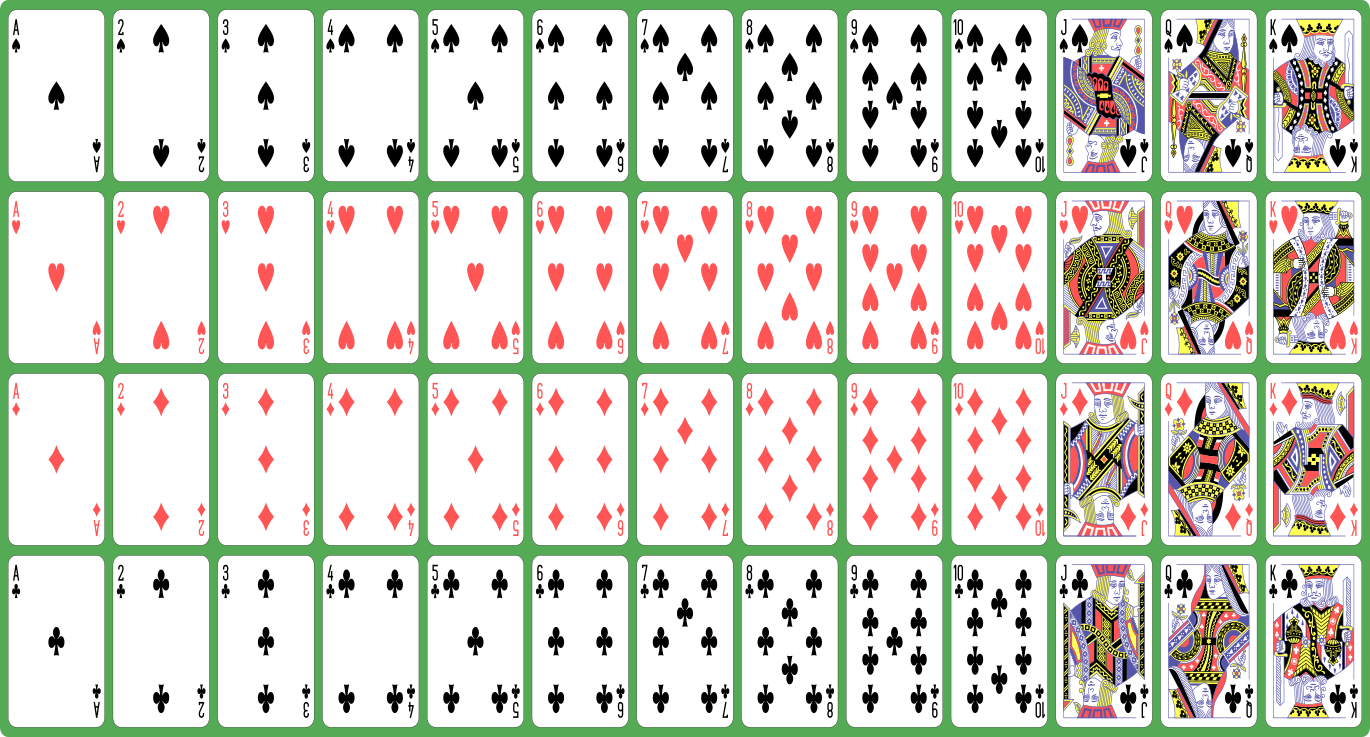
\includegraphics[width=0.8\linewidth,clip=]{images/poker_playing_cards.png}%
	\figcaption{Izgled igračih karata za poker}%
	\label{fig:poker_cards}%
\end{minipage}
\\[\intextsep]

Ruke poredane od najslabije do najjače:
\begin{itemize}
	\item Visoka karta (eng. \textit{high card}): Igrač nije uspijo složiti odgovarajuće kombinacije i gleda se karta sa najjačon vrijednosti. Karte poredane po jačini (od najslabije prema najjače):
	brojevi od 2 do 10 (veći broj znači snažnija karta), dečko, kraljica, kralj pa as.
	
	\item Par (eng. \textit{pair}): Igrač od bilo koje vrijednosti je uspio skupiti dvije iste.
	\item Dva para (eng. \textit{two pairs}): Ruka se sastoji od dvije karte s jednom vrijdnosti i dvije s drugom.
	\item Tris (eng. \textit{tris}): Bilo koja vrijednost 3 puta.
	\item Skala (eng. \textit{straight}): Pet različitih vrijednosti od tako da je svaka sljedeća karta za jednu vrijednost jača od prethodne.
	
	\item Boja (eng. \textit{flush}): Pet karte istog simbola.
	\item Puna kuća (eng. \textit{full house}): Tri karte iste vrijednosti i dvije druge karte istih vrijednosti.
	\item Poker (eng. \textit{poker}): Četiri karte istih vrijednosti.
	\item Skala u boji(eng. \textit{straight flush}): Pet vrijednosti gdje je svaka slijedeća za jednu vrijednost jača od predhodne i svi u istim simbolima.
	
	\item Kraljevska skala u boji (eng. \textit{royal flush}): 10, dečko, kraljica, kralj, as u istim simbolima.
\end{itemize}

\subsection{Pravila igre}
Igra koja se implementirala se naziva \emph{Limit Texas hold'em tournament}, i pravila su sljedeća. 
Potrebno je bar dva igrača, tri da bude zanimljivo pa do nekih desetak (nema neke fiksne gornje granice, 
ali najčešće je deset). Prije početka igre svi igrači uplaćuju dogovoreni iznos novca za sudjelovanje u igri, te dobije za uzvrat žetone vrijednosti uloženog novca. Igrači sjedu za ovalnim stolom i jednega od igrača se određuje kao diler. Diler dobije poseban žeton koji ga vidljivo označava kao takvog. Karte se izmišaju i svakom igraču se dodjeli dvije karte, u smjeru kazaljke na satu. Ove dvije karte su za ostale igrače tajna, znači svaki igrač nastoji da jedini vidi te karte, zapamti ih i po mogućnosti do kraja kruga ih drži okrenute naopako na stolu. U prvoj fazi \emph{pre flop} nakon djeljenje karata prvi igrač lijevo od dilera je prisiljen uložit žetone u visini pola vrijednosti minimalnog uloga, taj ulog se naziva \emph{small blind}, a slijedeći ulaže \emph{big blind} cijelokupan minimalni ulog, također prisiljeno. Prisiljeni ulozi služe kako bi u svakom krugu postojala neka dobit, a i da skrati igru koja i onako zna potrajati satima. Ostali igrači nakon njih imaju mogućnost birat hoće pratit (eng. \textit{call}), znači da moraju sve skupa uložit koliki je trenutačni največi ulog, dali će odustat i preklope karte (eng. \textit{fold}), gdje odbacuju karte iz ruku i izključeni su iz igre do kraja kruga ili će povisiti (eng. \textit{raise}) ulog, u kojem slučaju trenutačni ulog postane jednak prošlom plus minimalni iznos za ulaganje. U trenutku kada su ostali igrači napravili potez, prvi igrač do dilera mora nadoplatit ostali isnos za pratit ili izabrat neki od drugih poteza i na kraju igrač koji je mora prisilno uložit minimalni ulog ima mogućnost napravit potez, s tim ako nije bilo povisivanje uloga umisto pratit (eng. \textit{call}) ima potez potvrde (eng. \textit{check}), što znači da nema namjeru povisiti ulog niti izostat iz trenutačnog kruga. Kada svi igrači potvrdu potez diler izbacuje jednu kartu iz igre, reče se da se karta gori (eng. \textit{burn}), te na srid stola okrene 3 karte vidljive svima, to je \emph{flop} faza. 
Karte okrenute na srid stola su karte zajednice (eng. \textit{community cards}) i svaki igrač ima pravo svoju ruku od pet karata složit sa bilo kakvom kombinacijom svoje vlastite ruke i kartama zajednice. Slijedi potez svakog igrača, međutim u ostalim fazama nema prislinog ulaganja. U \emph{turn} fazi diler opet izbacuje kartu i okrene sljedeću na stol, ponovno svi igrači određuju svoji potezi. \emph{River} faza je identična \emph{turn} fazi, tako da na kraju su pet karte okrenuti na sredini stola i bar dva igrača u igri. Sada igrači okreću karte i izjasnu koju kombinaciju su sebi složili, i igrač sa najjačon kombinacijon kupi ukupan ulog (eng. \textit{pot}), ili ako imaju nekoliko igrači istu jačinu onda ga djele. Ako se u bilo kojoj fazi dogodi da svi osim jednog igrača odustaju, preskaču se ostale faze i igrač skuplja ukupni ulog. Postoji još poseban potez ulaganja sve (eng. \textit{all in}) gdje igrač kada nema dovoljno žetonih za uložit, ulaže sve što ima i u slučaju gubitka izbačen je iz igre. Dobitnik je igrač koji zadnji ostaje u igri i nagrada mu ukupan uplaćeni ulog svih igrača. Pošto je igra nepotpuno informirana igra postoji mogućnost blefiranja gdje igrač sa lošom rukom ulaže i/ili diže ulog da stvori dojam da ima jaku ruku na račun kojeg će neki ili svi ostali igrači odustati u trenutačnom krugu.


\emph{Limit} označava da je svaki ulog fiksan i u svakoj fazi su dozvoljena tri ponovno povisivanje uloga (eng. \textit{reraise}), gdje za razliku od \emph{no limit} igrač može povisiti najmanje minimalan ulog a najviše koliko hoće te nema ograničen broj ponovnog povisivanje uloga.

\emph{Texas hold'em} je ovaj način igre sa dvije tajnim kartama i pet javnih, gdje u klasičnom pokeru svaki igrač dobije pet karte (koje su drugim igračima tajna) im pravo izbacit nijednu, nekoliko ili sve karte i onoliko koliko je izbaci dobije novih, te postaje konačna ruka.

\emph{Tournament} podrazumjeva da svi igrači na početku uplate jednak iznos i igra se dok svi ispadnu osim jednog, dok u \emph{cash game} može igrač ponovno kupit žetone za nastavit igrat, može odustat od igre 
iako nije izgubi sve žetone te ih unovčit mogu i čak naknadno doć novi igrači.